\section{Principles}

\begin{frame}
\frametitle{Set your goals}
\begin{columns}
    \column{0.75\textwidth}
    \begin{itemize}
	\item Reducing boot time implies measuring boot time!
	\item You will have to choose reference events at which you
	      start and stop counting time.
	\item What you choose will depend on the goal you want to
              achieve. Here are typical cases:
	\begin{itemize}
		\item Showing a splash screen or an animation, playing a sound to
	              indicate the board is booting
		\item Starting a listening service to handle a particular
	              message
	        \item Being fully functional as fast as possible
	\end{itemize}
    \end{itemize}
    \column{0.25\textwidth}
    % From http://openclipart.org/detail/46075/stop-watch-by-klaasvangend
    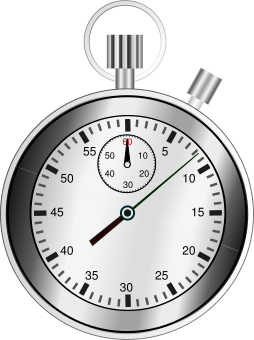
\includegraphics[width=\textwidth]{slides/boot-time-principles/stop-watch.pdf}
  \end{columns}
\end{frame}

\begin{frame}
\frametitle{Boot time reduction methodology}
\begin{center}
    \includegraphics[width=\textwidth]{slides/boot-time-principles/methodology.pdf}
\end{center}
\end{frame}

\begin{frame}
\frametitle{Boot time components}
\begin{center}
    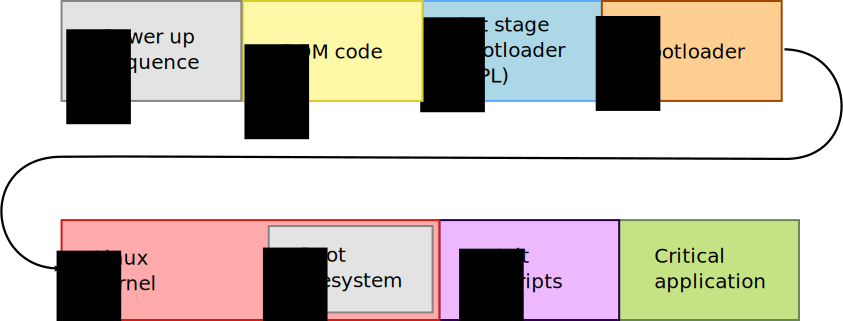
\includegraphics[width=\textwidth]{slides/boot-time-principles/generic-boot-sequence.pdf}
\end{center}
We are focusing on reducing {\em cold} boot time, from power on to the
critical application.
\end{frame}

\begin{frame}
\frametitle{What to optimize first}
Start by optimizing the {\bf last steps} of the boot process!
\begin{itemize}
\item Don't start by optimizing things that will reduce your ability to
      make measurements and implement other optimizations.
\item Start by optimizing your applications and startup
      scripts first.
\item You can then simplify BusyBox, reducing the number of available
      commands.
\item The next thing to do is simplify and optimize the kernel. This
      will make you lose debugging and development capabilities,
      but this is fine as user space has already been simplified.
\item The last thing to do is implement bootloader optimizations,
      when kernel optimizations are over and when the kernel command
      line is frozen.
\end{itemize}
We will follow this order during the practical labs.
\end{frame}

\begin{frame}
\frametitle{Worst things first!}
{\em Premature optimization is the root of all evil.\\
Donald Knuth}
\begin{itemize}
\item Taking the time to measure time carefully is important.
\item Find the worst consumers of time and address them first.
\item You can waste a lot of time if you start optimizing
      minor spots first.
\end{itemize}
\end{frame}

\begin{frame}
\frametitle{Build automation}
\begin{itemize}
\item Very important to automate the way the root filesystem is built,
      if not done yet. That's always the first thing we do in boot time
      reduction projects, and it's worth investing 1 or 2 days doing
      this.
\item Otherwise, you may lose existing optimizations or introduce new bugs
      when making further optimizations. Without a build system,
      you will waste a lot of time too.
\item Can be done through build systems such as Buildroot or Yocto,
      or using the original build automation of the project.
\item Can also be done for kernel and bootloader optimizations, though
      the need is less critical.
\end{itemize}
\end{frame}

\begin{frame}
\frametitle{Generic ideas}
Some ideas to keep in mind while trying to reduce the boot time:
\begin{itemize}
\item The fastest code is code that is not executed
\item A big part of booting is actually loading code and data from the
      storage to RAM. Reading less means booting faster. I/O are
      expensive!
\item The root filesystem may take longer to mount if it is bigger.
\item So, even code that is not executed can make your boot time
      longer.
\item Also, try to benchmark different types of storage. It has
      happened that booting from SD card was actually faster than
      booting from NAND.
\end{itemize}
\end{frame}
